

\tikzset{every picture/.style={line width=0.75pt}} %set default line width to 0.75pt        

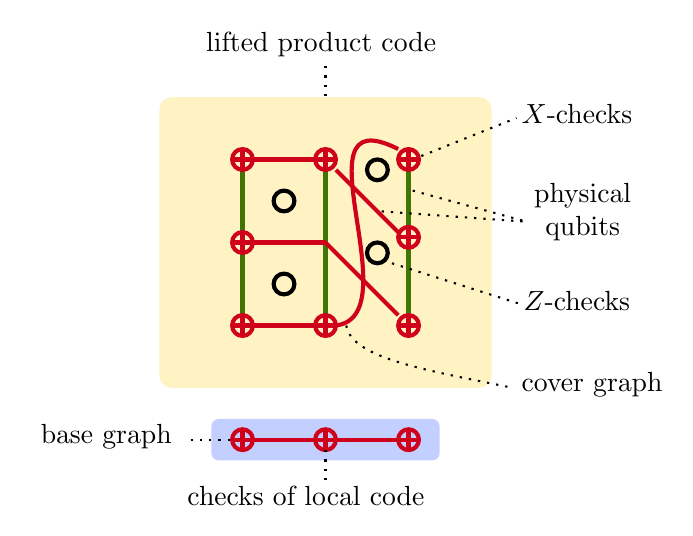
\begin{tikzpicture}[x=0.75pt,y=0.75pt,yscale=-1,xscale=1]
%uncomment if require: \path (0,275); %set diagram left start at 0, and has height of 275

%Rounded Rect [id:dp04206681589479189] 
\draw  [draw opacity=0][fill={rgb, 255:red, 194; green, 206; blue, 255 }  ,fill opacity=0.99 ] (185,228.6) .. controls (185,226.61) and (186.61,225) .. (188.6,225) -- (291.4,225) .. controls (293.39,225) and (295,226.61) .. (295,228.6) -- (295,241.4) .. controls (295,243.39) and (293.39,245) .. (291.4,245) -- (188.6,245) .. controls (186.61,245) and (185,243.39) .. (185,241.4) -- cycle ;
%Rounded Rect [id:dp19668680266647875] 
\draw  [draw opacity=0][fill={rgb, 255:red, 255; green, 243; blue, 194 }  ,fill opacity=0.99 ] (160,75.75) .. controls (160,72.58) and (162.58,70) .. (165.75,70) -- (314.25,70) .. controls (317.42,70) and (320,72.58) .. (320,75.75) -- (320,204.25) .. controls (320,207.42) and (317.42,210) .. (314.25,210) -- (165.75,210) .. controls (162.58,210) and (160,207.42) .. (160,204.25) -- cycle ;
%Straight Lines [id:da39257503404908944] 
\draw [color={rgb, 255:red, 65; green, 117; blue, 5 }  ,draw opacity=1 ][line width=1.5]    (200,100) -- (200,180) ;
%Straight Lines [id:da5680703852721674] 
\draw [color={rgb, 255:red, 65; green, 117; blue, 5 }  ,draw opacity=1 ][line width=1.5]    (240,100) -- (240,180) ;
%Straight Lines [id:da26529916700403366] 
\draw [color={rgb, 255:red, 65; green, 117; blue, 5 }  ,draw opacity=1 ][line width=1.5]    (280,100) -- (280,185) ;
%Shape: Circle [id:dp6526274403761385] 
\draw  [line width=1.5]  (215,120) .. controls (215,117.24) and (217.24,115) .. (220,115) .. controls (222.76,115) and (225,117.24) .. (225,120) .. controls (225,122.76) and (222.76,125) .. (220,125) .. controls (217.24,125) and (215,122.76) .. (215,120) -- cycle ;
%Shape: Circle [id:dp9203872961896724] 
\draw  [line width=1.5]  (260,145) .. controls (260,142.24) and (262.24,140) .. (265,140) .. controls (267.76,140) and (270,142.24) .. (270,145) .. controls (270,147.76) and (267.76,150) .. (265,150) .. controls (262.24,150) and (260,147.76) .. (260,145) -- cycle ;
%Shape: Circle [id:dp36121698938520197] 
\draw  [line width=1.5]  (215,160) .. controls (215,157.24) and (217.24,155) .. (220,155) .. controls (222.76,155) and (225,157.24) .. (225,160) .. controls (225,162.76) and (222.76,165) .. (220,165) .. controls (217.24,165) and (215,162.76) .. (215,160) -- cycle ;
%Straight Lines [id:da7945218011813688] 
\draw [color={rgb, 255:red, 208; green, 2; blue, 27 }  ,draw opacity=1 ][line width=1.5]    (200,235) -- (285,235) ;
%Straight Lines [id:da12955761798321674] 
\draw  [dash pattern={on 0.84pt off 2.51pt}]  (282,100) -- (332,80) ;
%Straight Lines [id:da7916884968167328] 
\draw  [dash pattern={on 0.84pt off 2.51pt}]  (272,150) -- (335,170) ;
%Straight Lines [id:da5071726340407701] 
\draw  [dash pattern={on 0.84pt off 2.51pt}]  (267,125) -- (337,130) ;
%Straight Lines [id:da11661211709797947] 
\draw  [dash pattern={on 0.84pt off 2.51pt}]  (282,115) -- (337,130) ;
%Straight Lines [id:da9782521186746413] 
\draw  [dash pattern={on 0.84pt off 2.51pt}]  (175,235) -- (195,235) ;
%Straight Lines [id:da2771657515983157] 
\draw  [dash pattern={on 0.84pt off 2.51pt}]  (240,55) -- (240,70) ;
%Straight Lines [id:da5295130285898282] 
\draw [color={rgb, 255:red, 208; green, 2; blue, 27 }  ,draw opacity=1 ][line width=1.5]    (245,105) -- (275,135) ;
%Curve Lines [id:da4557441417707939] 
\draw [color={rgb, 255:red, 208; green, 2; blue, 27 }  ,draw opacity=1 ][line width=1.5]    (275,95) .. controls (221.5,67.75) and (287,184.3) .. (240,180) ;
%Straight Lines [id:da4576616911447722] 
\draw [color={rgb, 255:red, 208; green, 2; blue, 27 }  ,draw opacity=1 ][line width=1.5]    (200,180) -- (240,180) ;
%Straight Lines [id:da5337345046576101] 
\draw [color={rgb, 255:red, 208; green, 2; blue, 27 }  ,draw opacity=1 ][line width=1.5]    (200,140) -- (240,140) ;
%Straight Lines [id:da6056724072089152] 
\draw [color={rgb, 255:red, 208; green, 2; blue, 27 }  ,draw opacity=1 ][line width=1.5]    (200,100) -- (240,100) ;
%Straight Lines [id:da8080159264893862] 
\draw [color={rgb, 255:red, 208; green, 2; blue, 27 }  ,draw opacity=1 ][fill={rgb, 255:red, 255; green, 0; blue, 0 }  ,fill opacity=1 ][line width=1.5]    (240,140) -- (275,175) ;
%Curve Lines [id:da7138097153136329] 
\draw  [dash pattern={on 0.84pt off 2.51pt}]  (250,180) .. controls (252.6,196.1) and (290.2,201.7) .. (330,210) ;
%Flowchart: Or [id:dp25442593723296913] 
\draw  [color={rgb, 255:red, 208; green, 2; blue, 27 }  ,draw opacity=1 ][line width=1.5]  (195,235) .. controls (195,232.24) and (197.24,230) .. (200,230) .. controls (202.76,230) and (205,232.24) .. (205,235) .. controls (205,237.76) and (202.76,240) .. (200,240) .. controls (197.24,240) and (195,237.76) .. (195,235) -- cycle ; \draw  [color={rgb, 255:red, 208; green, 2; blue, 27 }  ,draw opacity=1 ][line width=1.5]  (195,235) -- (205,235) ; \draw  [color={rgb, 255:red, 208; green, 2; blue, 27 }  ,draw opacity=1 ][line width=1.5]  (200,230) -- (200,240) ;
%Flowchart: Or [id:dp34071271062210373] 
\draw  [color={rgb, 255:red, 208; green, 2; blue, 27 }  ,draw opacity=1 ][line width=1.5]  (235,235) .. controls (235,232.24) and (237.24,230) .. (240,230) .. controls (242.76,230) and (245,232.24) .. (245,235) .. controls (245,237.76) and (242.76,240) .. (240,240) .. controls (237.24,240) and (235,237.76) .. (235,235) -- cycle ; \draw  [color={rgb, 255:red, 208; green, 2; blue, 27 }  ,draw opacity=1 ][line width=1.5]  (235,235) -- (245,235) ; \draw  [color={rgb, 255:red, 208; green, 2; blue, 27 }  ,draw opacity=1 ][line width=1.5]  (240,230) -- (240,240) ;
%Flowchart: Or [id:dp11995328939243666] 
\draw  [color={rgb, 255:red, 208; green, 2; blue, 27 }  ,draw opacity=1 ][line width=1.5]  (275,235) .. controls (275,232.24) and (277.24,230) .. (280,230) .. controls (282.76,230) and (285,232.24) .. (285,235) .. controls (285,237.76) and (282.76,240) .. (280,240) .. controls (277.24,240) and (275,237.76) .. (275,235) -- cycle ; \draw  [color={rgb, 255:red, 208; green, 2; blue, 27 }  ,draw opacity=1 ][line width=1.5]  (275,235) -- (285,235) ; \draw  [color={rgb, 255:red, 208; green, 2; blue, 27 }  ,draw opacity=1 ][line width=1.5]  (280,230) -- (280,240) ;
%Flowchart: Or [id:dp23233234623865284] 
\draw  [color={rgb, 255:red, 208; green, 2; blue, 27 }  ,draw opacity=1 ][line width=1.5]  (195,180) .. controls (195,177.24) and (197.24,175) .. (200,175) .. controls (202.76,175) and (205,177.24) .. (205,180) .. controls (205,182.76) and (202.76,185) .. (200,185) .. controls (197.24,185) and (195,182.76) .. (195,180) -- cycle ; \draw  [color={rgb, 255:red, 208; green, 2; blue, 27 }  ,draw opacity=1 ][line width=1.5]  (195,180) -- (205,180) ; \draw  [color={rgb, 255:red, 208; green, 2; blue, 27 }  ,draw opacity=1 ][line width=1.5]  (200,175) -- (200,185) ;
%Flowchart: Or [id:dp40821844186146516] 
\draw  [color={rgb, 255:red, 208; green, 2; blue, 27 }  ,draw opacity=1 ][line width=1.5]  (235,180) .. controls (235,177.24) and (237.24,175) .. (240,175) .. controls (242.76,175) and (245,177.24) .. (245,180) .. controls (245,182.76) and (242.76,185) .. (240,185) .. controls (237.24,185) and (235,182.76) .. (235,180) -- cycle ; \draw  [color={rgb, 255:red, 208; green, 2; blue, 27 }  ,draw opacity=1 ][line width=1.5]  (235,180) -- (245,180) ; \draw  [color={rgb, 255:red, 208; green, 2; blue, 27 }  ,draw opacity=1 ][line width=1.5]  (240,175) -- (240,185) ;
%Flowchart: Or [id:dp8091211396517879] 
\draw  [color={rgb, 255:red, 208; green, 2; blue, 27 }  ,draw opacity=1 ][line width=1.5]  (275,180) .. controls (275,177.24) and (277.24,175) .. (280,175) .. controls (282.76,175) and (285,177.24) .. (285,180) .. controls (285,182.76) and (282.76,185) .. (280,185) .. controls (277.24,185) and (275,182.76) .. (275,180) -- cycle ; \draw  [color={rgb, 255:red, 208; green, 2; blue, 27 }  ,draw opacity=1 ][line width=1.5]  (275,180) -- (285,180) ; \draw  [color={rgb, 255:red, 208; green, 2; blue, 27 }  ,draw opacity=1 ][line width=1.5]  (280,175) -- (280,185) ;
%Flowchart: Or [id:dp3594142462274845] 
\draw  [color={rgb, 255:red, 208; green, 2; blue, 27 }  ,draw opacity=1 ][line width=1.5]  (275,137.5) .. controls (275,134.74) and (277.24,132.5) .. (280,132.5) .. controls (282.76,132.5) and (285,134.74) .. (285,137.5) .. controls (285,140.26) and (282.76,142.5) .. (280,142.5) .. controls (277.24,142.5) and (275,140.26) .. (275,137.5) -- cycle ; \draw  [color={rgb, 255:red, 208; green, 2; blue, 27 }  ,draw opacity=1 ][line width=1.5]  (275,137.5) -- (285,137.5) ; \draw  [color={rgb, 255:red, 208; green, 2; blue, 27 }  ,draw opacity=1 ][line width=1.5]  (280,132.5) -- (280,142.5) ;
%Flowchart: Or [id:dp1885881339588107] 
\draw  [color={rgb, 255:red, 208; green, 2; blue, 27 }  ,draw opacity=1 ][line width=1.5]  (275,100) .. controls (275,97.24) and (277.24,95) .. (280,95) .. controls (282.76,95) and (285,97.24) .. (285,100) .. controls (285,102.76) and (282.76,105) .. (280,105) .. controls (277.24,105) and (275,102.76) .. (275,100) -- cycle ; \draw  [color={rgb, 255:red, 208; green, 2; blue, 27 }  ,draw opacity=1 ][line width=1.5]  (275,100) -- (285,100) ; \draw  [color={rgb, 255:red, 208; green, 2; blue, 27 }  ,draw opacity=1 ][line width=1.5]  (280,95) -- (280,105) ;
%Flowchart: Or [id:dp3230896903801863] 
\draw  [color={rgb, 255:red, 208; green, 2; blue, 27 }  ,draw opacity=1 ][line width=1.5]  (235,100) .. controls (235,97.24) and (237.24,95) .. (240,95) .. controls (242.76,95) and (245,97.24) .. (245,100) .. controls (245,102.76) and (242.76,105) .. (240,105) .. controls (237.24,105) and (235,102.76) .. (235,100) -- cycle ; \draw  [color={rgb, 255:red, 208; green, 2; blue, 27 }  ,draw opacity=1 ][line width=1.5]  (235,100) -- (245,100) ; \draw  [color={rgb, 255:red, 208; green, 2; blue, 27 }  ,draw opacity=1 ][line width=1.5]  (240,95) -- (240,105) ;
%Flowchart: Or [id:dp2944443388643656] 
\draw  [color={rgb, 255:red, 208; green, 2; blue, 27 }  ,draw opacity=1 ][line width=1.5]  (195,140) .. controls (195,137.24) and (197.24,135) .. (200,135) .. controls (202.76,135) and (205,137.24) .. (205,140) .. controls (205,142.76) and (202.76,145) .. (200,145) .. controls (197.24,145) and (195,142.76) .. (195,140) -- cycle ; \draw  [color={rgb, 255:red, 208; green, 2; blue, 27 }  ,draw opacity=1 ][line width=1.5]  (195,140) -- (205,140) ; \draw  [color={rgb, 255:red, 208; green, 2; blue, 27 }  ,draw opacity=1 ][line width=1.5]  (200,135) -- (200,145) ;
%Flowchart: Or [id:dp6176631813922029] 
\draw  [color={rgb, 255:red, 208; green, 2; blue, 27 }  ,draw opacity=1 ][line width=1.5]  (195,100) .. controls (195,97.24) and (197.24,95) .. (200,95) .. controls (202.76,95) and (205,97.24) .. (205,100) .. controls (205,102.76) and (202.76,105) .. (200,105) .. controls (197.24,105) and (195,102.76) .. (195,100) -- cycle ; \draw  [color={rgb, 255:red, 208; green, 2; blue, 27 }  ,draw opacity=1 ][line width=1.5]  (195,100) -- (205,100) ; \draw  [color={rgb, 255:red, 208; green, 2; blue, 27 }  ,draw opacity=1 ][line width=1.5]  (200,95) -- (200,105) ;
%Shape: Circle [id:dp6429784049874268] 
\draw  [line width=1.5]  (260,105) .. controls (260,102.24) and (262.24,100) .. (265,100) .. controls (267.76,100) and (270,102.24) .. (270,105) .. controls (270,107.76) and (267.76,110) .. (265,110) .. controls (262.24,110) and (260,107.76) .. (260,105) -- cycle ;
%Straight Lines [id:da5104559986502026] 
\draw  [dash pattern={on 0.84pt off 2.51pt}]  (240,240) -- (240,255) ;

% Text Node
\draw (179,37) node [anchor=north west][inner sep=0.75pt]   [align=left] {\begin{minipage}[lt]{86.07304pt}\setlength\topsep{0pt}
\begin{center}
lifted product code
\end{center}

\end{minipage}};
% Text Node
\draw (97,226) node [anchor=north west][inner sep=0.75pt]   [align=left] {\begin{minipage}[lt]{53.7625pt}\setlength\topsep{0pt}
\begin{center}
base graph
\end{center}

\end{minipage}};
% Text Node
\draw (333,72) node [anchor=north west][inner sep=0.75pt]   [align=left] {$\displaystyle X$-checks};
% Text Node
\draw (334,162) node [anchor=north west][inner sep=0.75pt]   [align=left] {$\displaystyle Z$-checks};
% Text Node
\draw (336,110) node [anchor=north west][inner sep=0.75pt]   [align=left] {\begin{minipage}[lt]{39.578108pt}\setlength\topsep{0pt}
\begin{center}
physical\\qubits
\end{center}

\end{minipage}};
% Text Node
\draw (333,201) node [anchor=north west][inner sep=0.75pt]   [align=left] {cover graph};
% Text Node
\draw (172,256) node [anchor=north west][inner sep=0.75pt]   [align=left] {checks of local code};


\end{tikzpicture}
